\documentclass[9pt, aspectratio=169]{beamer}

\usetheme{metropolis}
\setbeamertemplate{itemize items}{\faAngleRight}

\metroset{titleformat=smallcaps,block=fill,numbering=counter,progressbar=frametitle,sectionpage=none}
\setbeamersize{text margin left=5mm,text margin right=5mm} 
% \input{embed_video}
\usepackage{fontspec,minted}
\usepackage[scale=1]{ccicons}
\usepackage{metalogo}
\usepackage{xcolor,colortbl}
\usepackage{multicol,multirow,booktabs}
\usepackage{appendixnumberbeamer}
\usepackage{graphicx}
\usepackage{mismath}
\usepackage{bm}
\usepackage{fontawesome5}
\usepackage{csquotes}
%\usepackage[backend=biber, natbib, sorting=nyt, doi=true, url=false, url=false, isbn=false, maxbibnames=10]{biblatex}
%\addbibresource{../../utils/refs.bib}

\usepackage[spanish, es-nodecimaldot]{babel}
\deftranslation[to=spanish]{Definition}{Definición}
\deftranslation[to=spanish]{Theorem}{Teorema}
\deftranslation[to=spanish]{Example}{Ejemplo}

\usepackage{mathtools, mathrsfs}
\usefonttheme{professionalfonts}
\usepackage{textcomp, wasysym}

\setsansfont[BoldFont={Iwona Bold}, Numbers={Lining, Proportional}]{Iwona Light}
% \setmathsfont(Digits)[Numbers={Lining, Proportional}]{Fira Sans Light}
\setmonofont[Scale=MatchLowercase]{DejaVu Sans Mono}

\setbeamercolor{alerted text}{fg=red,bg=black!2}
\setbeamercolor{progress bar}{fg=red,bg=red!2}
\setbeamertemplate{itemize item}{\faCaretRight}
\setbeamertemplate{itemize subitem}{ \faAngleRight}
\setbeamertemplate{blocks}[shadow=false]
\setbeamercolor{block title}{bg=black!30,fg=red}
\setbeamercolor{block body}{bg=black!20,fg=black}
\setbeamertemplate{theorem begin}
{%
\begin{\inserttheoremblockenv}
{%
\inserttheoremheadfont
%{Teorema:}
\inserttheoremname
\ifx\inserttheoremaddition\@empty\else\ : \inserttheoremaddition\fi%
\inserttheorempunctuation
}%
}
\setbeamertemplate{theorem end}{\end{\inserttheoremblockenv}}
\makeatother


 
\usepackage{gensymb,amssymb}
\usepackage{upquote}
\usepackage{cancel}
\usepackage{algpseudocode}
\algrenewcommand\algorithmicrequire{\textbf{Requiere}}
\algrenewcommand\algorithmicensure{\textbf{Devuelve}}
\setbeamertemplate{blocks}[shadow=false]

\newcommand{\cx}{\column{0.5\textwidth}}
\newcommand{\cw}[1]{\column{#1\textwidth}}

\author{Manuel Carlevaro}
\date{}
\institute{
  \vspace{6em}
  \centering
  {\tiny
  Universidad de Navarra \enspace • \enspace 2024 
} }

%% Operadores
\DeclareMathOperator{\sen}{sen}
\DeclareMathOperator{\senc}{senc}
\DeclareMathOperator{\sign}{sign}
\newcommand{\T}[1]{\underline{\bm{#1}}}
\DeclareMathOperator{\Tr}{Tr}
\DeclareMathOperator{\rg}{rg}
\DeclareMathOperator{\cond}{cond}

\usepackage{hyperref}
\hypersetup{
    colorlinks,
    citecolor=blue,
    filecolor=black,
    linkcolor=blue,
    urlcolor=blue
}
\urlstyle{same}


\usepackage{tikz}
\usetikzlibrary{shapes,shadows,arrows,positioning,matrix,chains,backgrounds,fit}

\tikzset{
    %Define standard arrow tip
    >=stealth',
    %Define style for boxes
    obj/.style={
           rectangle,
           rounded corners,
           draw, very thick,
           text width=10em, fill=green!20,
           minimum height=2em,
           text centered, drop shadow},
    proc/.style={
	    rectangle, rounded corners,
	    draw,fill=red!50,very thick,
	    text width=8em,minimum height=2em,
	    text centered, drop shadow},
    % Define arrow style
    pil/.style={
           ->,
           thick,
           shorten <=2pt,
           shorten >=2pt,}
}

%\setbeamertemplate{bibliography item}{%
  %\ifboolexpr{ test {\ifentrytype{book}} or test {\ifentrytype{mvbook}}
    %or test {\ifentrytype{collection}} or test {\ifentrytype{mvcollection}}
    %or test {\ifentrytype{reference}} or test {\ifentrytype{mvreference}} }
    %{\setbeamertemplate{bibliography item}{\faBook}}
    %{\ifentrytype{online}
            %{\setbeamertemplate{bibliography item}{\faGlobe}}
   %{\setbeamertemplate{bibliography item}{\faFileText}}}%
  %\usebeamertemplate{bibliography item}}

%\defbibenvironment{bibliography}
  %{\list{}
     %{\settowidth{\labelwidth}{\usebeamertemplate{bibliography item}}%
      %\setlength{\leftmargin}{\labelwidth}%
      %\setlength{\labelsep}{\biblabelsep}%
      %\addtolength{\leftmargin}{\labelsep}%
      %\setlength{\itemsep}{\bibitemsep}%
      %\setlength{\parsep}{\bibparsep}}}
  %{\endlist}
  %{\item}
%\newcommand{\bcite}[1]{\citeauthor{#1}, \citetitle{#1} (\citeyear{#1})}


\title{Introducción a las matemáticas}
\subtitle{Conjuntos numéricos}


\begin{document}
\maketitle

\begin{frame}{ Objetivos }
\begin{multicols}{2}
\begin{itemize}
    \item Definir conjuntos por extensión y comprensión. Realizar diagramas de Venn. Identificar elementos y subconjuntos a la vez que relaciones de pertenencia e inclusión.
    \item Realizar operaciones entre conjuntos (unión, intersección y diferencia).
    \item Identificar los conjuntos numéricos.
    \item Revisar la conformación de los números reales: números naturales, enteros, racionales e irracionales.
    \item Conocer la representación del conjunto de los números reales como recta real y los demás conjuntos numéricos.
\item Revisar cómo se manipulan expresiones algebraicas usando las propiedades conmutativas, asociativas y distributivas de las operaciones.
\item Conocer el orden de las prioridades de las operaciones algebraicas y el rol de los paréntesis.
\item Revisar identidades algebraicas importantes que involucran la suma, resta, multiplicación y división.
\end{itemize}
\end{multicols}
\end{frame}

\section{Conjuntos y operaciones entre conjuntos}
\subsection{Definiciones y relaciones de pertenencia e inclusión}

\begin{frame}{Conjuntos y operaciones entre conjuntos}
\begin{definition}[Conjunto]
        Es una colección o agrupamiento de objetos, cosas, etc. Usualmente se utilizan letras mayúsculas para nombrarlos y llaves $\{\}$ para \textbf{escribirlos encerrando sus elementos}.
\end{definition} 
\pause

\begin{example}
\[ S = \{ \text{domingo}, \text{martes}, \text{lunes}, \text{jueves}, \text{viernes}, \text{sábado}, \text{miércoles} \} \]
\end{example} \pause

\textbf{Otros ejemplos:}
\[ A = \{ \text{a}, \text{e}, \text{i}, \text{o}, \text{u} \} \quad B = \{ \text{rojo}, \text{verde}, \text{azul} \} \quad C = \{ \square, \ocircle, \triangle, \diamondsuit, \clubsuit\} \quad  D  = \{1, 2, 3, 4, 5, 6,7 ,8, 9, 0 \}  \]
\pause

\begin{alertblock}{\centering \faInfoCircle}
    \begin{itemize}
        \item \alert{No importa} el orden en que escribimos los elementos de un conjunto.
        \item Tampoco es importante que aparezcan \alert{elementos repetidos}. Por ejemplo, los siguientes conjuntos son iguales:
            \[ \{ \text{a}, \text{b}, \text{c} \} = \{ \text{a}, \text{c}, \text{b}, \text{b}, \text{b} \} = \{ \text{b}, \text{a}, \text{c}, \text{a} \} \]
    \end{itemize}
\end{alertblock}
\end{frame}

\begin{frame}{Conjuntos y operaciones entre conjuntos}
\begin{columns}[t]
\cw{0.45} 
Se utiliza el símbolo ``$\in$'' para indicar que cierto elemento \textbf{pertenece} a un conjunto:
\[ \text{lunes} \in S \]
Se puede leer como ``lunes pertenece a ``$S$''.

Por otro lado, se utiliza el símbolo ``$\notin$'' para indicar que un elemento \textbf{no pertenece} a un conjunto, por ejemplos:
\[ \text{enero} \notin S \]

Cuando el conjunto tiene \textbf{muchos elementos}, o una \textbf{cantidad infinita} de elementos, se utilizan los \textbf{tres puntos} ``$\ldots$'':
\[ \{ \text{a}, \text{b}, \text{c}, \ldots, \text{x}, \text{y}, \text{z} \} \]
\[ \{0, 1, 2, 3, 4, \ldots \} \]
\pause

\cw{0.45}
\textbf{Diagramas de Venn:}
\vspace{1em}

\begin{center}
    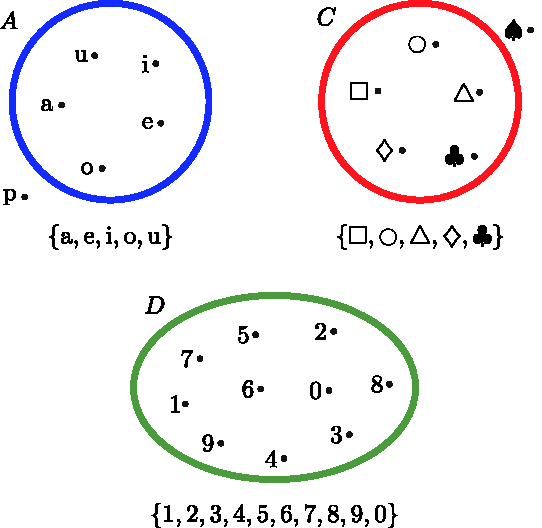
\includegraphics[width=1.0\textwidth]{figs/fig-01.pdf}
\end{center}

\end{columns}
\end{frame}

\begin{frame}{Conjuntos y operaciones entre conjuntos}
\begin{columns}[t]
\cw{0.5}
\begin{definition}[Conjunto vacío]
El conjunto que \textbf{no tiene elementos} se llama ``\textbf{conjunto vacío}'' y se denota con el símbolo ``$\varnothing$'':
\[ \varnothing = \{\} \]
\end{definition}

Con los elementos de un conjunto se pueden formar otros conjuntos ``más pequeños'' que se llaman \textbf{subconjuntos}. Por ejemplo, con $A = \{ \text{a}, \text{e}, \text{i}, \text{o}, \text{u}\}$ se pueden formar varios subconjuntos:
    \begin{align*}
        & \{ \text{e}, \text{i}, \text{o} \} \quad \{ \text{a} \} \quad \{ \text{a}, \text{e} \} \quad \{ \text{i}, \text{u} \}\\
        &\{ \text{i}, \text{o}, \text{u} \} \quad \{ \text{o}, \text{u} \} \quad \{ \text{u}, \text{o}, \text{a}, \text{e} \} \quad \{ \text{o} \}
    \end{align*}
En palabras se dice, por ejemplo, que:
\[ \{ \text{a}, \text{i} \} \txt{es un subconjunto de} \{ \text{a}, \text{e}, \text{i}, \text{o}, \text{u}\} \]

\cw{0.5} o que
\[ \{ \text{a}, \text{i} \} \txt{está incluido en} \{ \text{a}, \text{e}, \text{i}, \text{o}, \text{u}\} \]

\begin{definition}[$A \subseteq B$]
Se escribe $A \subseteq B$ cuando \textbf{todos los elementos} del conjunto $A$ también son elementos del conjunto $B$. En cambio, se escribe $A \nsubseteq B$ cuando \textbf{algún elemento} de $A$ no es un elemento del conjunto $B$
\end{definition}
\begin{center}
    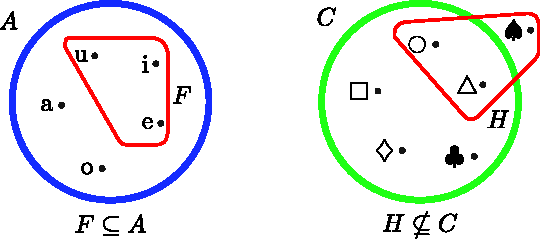
\includegraphics[width=1.0\textwidth]{figs/fig-02.pdf}
\end{center}

\end{columns}
\end{frame}

\begin{frame}{Conjuntos y operaciones entre conjuntos}
    Se puede describir a los conjuntos \textbf{por extensión} o \textbf{por comprensión}. Se dice que un conjunto está descripto por extensión cuando hacemos una lista de sus elementos, como en los ejemplos anteriores:

\[ A = \{ \text{a}, \text{e}, \text{i}, \text{o}, \text{u} \} \quad B = \{ \text{rojo}, \text{verde}, \text{azul} \} \quad C = \{ \square, \ocircle, \triangle, \diamondsuit, \clubsuit\} \quad  D  = \{1, 2, 3, 4, 5, 6,7 ,8, 9, 0 \}  \] 

Por otro lado, se dice que un conjunto está descripto por comprensión cuando se utiliza alguna propiedad característica de sus elementos, por ejemplo:
\[ A = \underbrace{\{ \text{el conjunto de las vocales} \}}_{\text{definición por comprensión}} = \underbrace{ \{ \text{a}, \text{e}, \text{i}, \text{o}, \text{u} \} }_{\text{definición por extensión}} \]

De manera más formal, se utiliza la siguiente notación para definir conjuntos por comprensión:
\[ A = \{ \underbrace{x \text{ es una letra}}_{\text{conjunto con el que trabajamos}} : \underbrace{x \text{ es una vocal}}_{\text{propiedad que debe cumplirse}} \} \]
Se lee: ``$A$ es el conjunto de las letras $x$ tal que $x$ es una vocal''. 
\end{frame}

\begin{frame}{Conjuntos y operaciones entre conjuntos}
\textbf{Ejemplos:}
    \begin{center}
        \begin{tabular}{p{9.5cm} p{4cm}}
            \toprule
            \textbf{Definición por comprensión} & \textbf{Definición por extensión} \\
            \midrule
            $\{ x : x \text{ es una letra de la palabra ``matemática''} \}$ & $\{$m, a, t, e, i , c$\}$ \\
            $\{ x : x \text{ es una vocal de la palabra ``matemática''}\}$ & $\{$a, e, i$\}$ \\
            $\{ x : x \text{ es un Estado miembro de la Unión Europea que empieza con ``F''}\}$ & $\{$Francia, Finlandia$\}$ \\
            $\{ x : x \text{ es un dígito decimal par}\}$ & $\{0, 2, 4, 6, 8\}$ \\
            \bottomrule
        \end{tabular}
    \end{center}

\vspace{3em}
\begin{center}
{\Large \faArrowCircleRight \faPen* Actividad 1}
\end{center}
\end{frame}

\subsection{Operaciones entre conjuntos}

\begin{frame}{Operaciones entre conjuntos}
\begin{columns}[c]
\cx
\begin{definition}[Intersección de conjuntos]
    La \textbf{intersección} de dos conjuntos es un nuevo conjunto formado por los elementos que están en ambos conjuntos simultáneamente. Considerando $A$ y $B$ dos conjuntos, escribimos la intersección de $A$ y $B$ de la siguiente forma:
    \[ A \cap B = \{ x : x \in A \text{ y } x \in B \} \]
\end{definition}

\begin{example}
    Si $A = \{$a, b, c, g$\}$ y $B = \{$r, g$\}$, entonces:
    \[ A \cap B = \{\text{g} \} \]
\end{example}

\cx
\begin{center}
    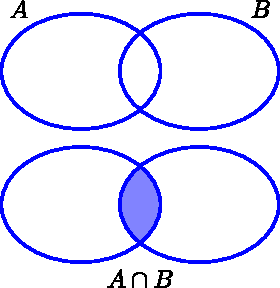
\includegraphics[scale=1.0]{figs/fig-03.pdf}
\end{center}
\end{columns}
\end{frame}

\begin{frame}{Operaciones entre conjuntos}
\begin{columns}[c]
\cx
\begin{definition}[Unión de conjuntos]
    La \textbf{unión} de dos conjuntos es un nuevo conjunto formado por los elementos que están en uno u otro conjunto. Considerando $A$ y $B$ dos conjuntos, escribimos la unión de $A$ y $B$ de la siguiente forma:
    \[ A \cup B = \{ x : x \in A \text{ o } x \in B \} \]
\end{definition}

\begin{example}
    Si $A = \{$a, b, c, g$\}$ y $B = \{$r, g$\}$, entonces:
    \[ A \cup B = \{\text{a}, \text{b}, \text{c}, \text{r}, \text{g} \} \]
\end{example}

\cx
\begin{center}
    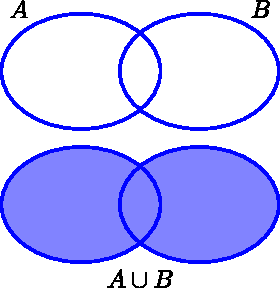
\includegraphics[scale=1.0]{figs/fig-04.pdf}
\end{center}
\end{columns}
\end{frame}

\begin{frame}{Operaciones entre conjuntos}
\begin{columns}[c]
\cx
\begin{definition}[Diferencia de conjuntos]
    La \textbf{diferencia} del conjunto $A$ con el conjunto $B$ es un nuevo conjunto formado por todos los elementos de $A$ que no están en $B$. Considerando $A$ y $B$ dos conjuntos, escribimos la diferencia de $A$ con $B$ de la siguiente forma:
    \[ A - B = \{ x : x \in A \text{ y } x \notin B \} \]
\end{definition}

\begin{example}
    Si $A = \{$a, b, c, g$\}$ y $B = \{$r, g$\}$, entonces:
    \[ A - B = \{\text{a}, \text{b}, \text{c} \} \]
\end{example}

\cx
\begin{center}
    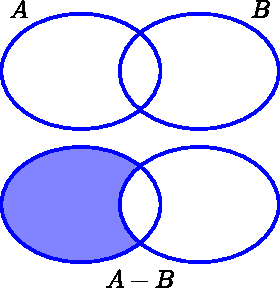
\includegraphics[scale=1.0]{figs/fig-05.pdf}
\end{center}
\end{columns}
\end{frame}

\begin{frame}{Operaciones entre conjuntos}
\begin{block}{Ejemplo:}
23 estudiantes de un curso practican alguno de los siguientes deportes: tenis, fútbol y voley. Cuatro de ellas juegan regularmente los tres deportes; 5 juegan solamente voley y fútbol; dos juegan solamente tenis y fútbol; y tres juegan solamente tenis y voley. Además, tres personas juegan únicamente tenis y una persona juega únicamente fútbol. ¿Cuantas personas juegan únicamente voley?
\vspace{-2.5em}
\begin{center}
\[ T = \{\text{estudiantes que juegan tenis}\}; V = \{\text{estudiantes que juegan voley}\}; F = \{\text{estudiantes que juegan fútbol}\} \]
\end{center}
\end{block} \pause
\begin{columns}[c]
\cw{0.6}
{\small
\begin{tabular}{ccc}
\toprule
\textbf{Enunciado} & \textbf{Conjunto} & \textbf{\# elementos} \\
\midrule
Total de alumnos & $V \cup F \cup T$ & 23 \\
Alumnos que juegan 3 deportes & $V \cap F \cap T$ & 4 \\
Alumnos que juegan únicamente voley y fútbol& $(V \cap F) - T$ & 5 \\
Alumnos que juegan únicamente tenis y fútbol& $(T \cap F) - V$ & 2 \\
Alumnos que juegan únicamente tenis y voley& $(T \cap V) - F$ & 3 \\
Alumnos que juegan únicamente tenis& $T - (V \cup F) $ & 3 \\
Alumnos que juegan únicamente fútbol& $F - (T \cup V) $ & 1 \\
Alumnos que juegan únicamente voley& $V - (T \cup F) $ & ¿? \\
\bottomrule
\end{tabular}
}
\cw{0.4}
\begin{center}
    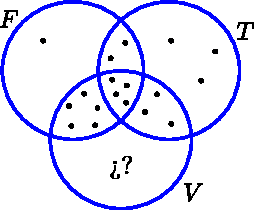
\includegraphics[scale=1.0]{figs/fig-06.pdf}
\end{center}
\end{columns}
\pause

\begin{center}
{\Large \faArrowCircleRight \faPen* Actividad 2}
\end{center}
\end{frame}





\end{document}

